\chapter{\ifproject%
\ifenglish Project Structure and Methodology\else โครงสร้างและขั้นตอนการทำงาน\fi
\else%
\ifenglish Project Structure\else โครงสร้างของโครงงาน\fi
\fi
}

\makeatletter

% \renewcommand\section{\@startsection {section}{1}{\z@}%
%                                    {13.5ex \@plus -1ex \@minus -.2ex}%
%                                    {2.3ex \@plus.2ex}%
%                                    {\normalfont\large\bfseries}}

\makeatother
%\vspace{2ex}
% \titleformat{\section}{\normalfont\bfseries}{\thesection}{1em}{}
% \titlespacing*{\section}{0pt}{10ex}{0pt}

\section{โครงสร้างทางสถาปัตยกรรม}

\begin{figure}[h]
\begin{center}
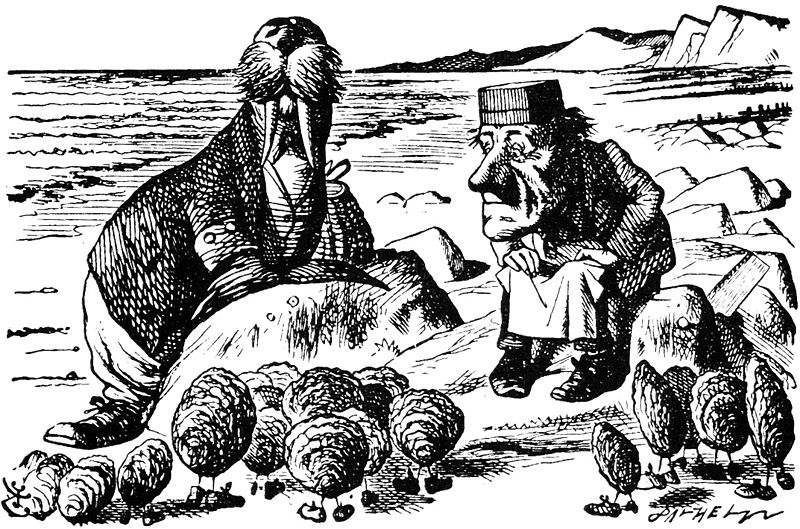
\includegraphics{800px-Briny_Beach.jpg}
\end{center}
\caption[Poem]{The Walrus and the Carpenter}
\label{fig:walrus}
\end{figure}

\section{การเตรียมข้อมูล (Data Preparation)}
\subsection{การโหลดและอ่านชุดข้อมูล (Data Loading)}
\hspace{2em} ขั้นตอนแรกคือการนำเข้าชุดข้อมูลที่ใช้สำหรับการทดลอง SWaT Dataset ซึ่งเป็นข้อมูลการทำงานของระบบน้ำในอุตสาหกรรมที่บันทึกค่า sensor และ actuator ในรูปแบบ time-series 
การโหลดข้อมูลอาจใช้เครื่องมืออย่าง Pandas เพื่ออ่านไฟล์ .csv แล้วจัดเก็บให้อยู่ในรูปแบบ DataFrame เพื่อให้สามารถจัดการได้สะดวกในขั้นตอนถัดไป

\subsection{การจัดการค่าที่หายไป (Missing Value Handling)}
\hspace{2em} ข้อมูลที่ได้จากระบบ OT/ICS มักมีปัญหาค่าที่หายไป (missing values) อันเนื่องมาจากปัญหาของ sensor หรือการบันทึกข้อมูล การจัดการอาจทำได้หลายวิธี เช่น
\begin{enumerate}
  \item การลบข้อมูลแถวที่หายไป (listwise deletion)
  \item การแทนค่าด้วยสถิติพื้นฐาน (เช่น ค่าเฉลี่ย ค่ามัธยฐาน)
  \item การแทนค่าด้วยการคำนวณจากข้อมูลรอบข้าง เช่น interpolation ในกรณีข้อมูลเชิงเวลา
\end{enumerate}

\subsection{การแยกประเภทคุณลักษณะ (Continuous / Discrete Features)}
\hspace{2em} ชุดข้อมูลมักประกอบด้วยคุณลักษณะหลายประเภท เช่น
\begin{enumerate}
  \item Continuous features: ค่าเซนเซอร์ เช่น ความดัน, อัตราการไหล
  \item Discrete features: ค่าสถานะ actuator เช่น เปิด/ปิดวาล์ว, เปิด/ปิดปั๊ม \\ การแยกประเภทคุณลักษณะมีความสำคัญเพราะวิธี preprocessing อาจแตกต่างกัน เช่น continuous ต้อง scaling แต่ discrete อาจใช้ encoding
\end{enumerate}

\subsection{การปรับสเกลข้อมูล (Scaling and Normalization)}
\hspace{2em} ค่าของเซนเซอร์บางตัวอาจอยู่ในช่วงที่ต่างกันมาก เช่น อุณหภูมิ (0–100) กับค่าแรงดัน (0–10,000) หากไม่ปรับสเกล อาจทำให้โมเดลให้ความสำคัญกับตัวแปรที่มีค่ามากเกินไป โดยใช้วิธี
\begin{center}
  Min-Max Scaling (ปรับให้อยู่ในช่วง [0,1])
\end{center}

\subsection{การแบ่งชุดข้อมูล (Training / Testing Split)}
\hspace{2em} เพื่อป้องกันการ overfitting ต้องแบ่งข้อมูลออกเป็น training set และ testing set เช่น 70/30 หรือ 80/20 ในงาน time-series อาจต้องใช้ sliding window ในการแบ่ง โดยไม่ทำการ shuffle ข้อมูล เพื่อคงลำดับเวลาให้ถูกต้อง

\section{การทำ Feature Engineering}

\subsection{การเลือกคุณลักษณะที่เกี่ยวข้อง (Feature Selection)}
\hspace{2em} ไม่ใช่ทุกคุณลักษณะมีความสำคัญต่อการตรวจจับ anomaly การใช้ feature selection จะช่วยลดมิติของข้อมูลและปรับปรุงประสิทธิภาพโมเดล เทคนิคที่ใช้เช่น
\begin{enumerate}
  \item การวิเคราะห์ Correlation Matrix
  \item การใช้ Mutual Information
  \item การใช้ Model-based feature selection เช่น Random Forest
\end{enumerate}


\subsection{การใช้ Sliding Window กับ Time-series Data}
\hspace{2em} เนื่องจากข้อมูล ICS/OT เป็น time-series จำเป็นต้องแปลงข้อมูลให้อยู่ในรูป window-based input เช่น สร้าง sequence ขนาด 30 หรือ 60 วินาที เพื่อใช้ในการเรียนรู้ pattern ของระบบ วิธีนี้ช่วยให้โมเดล CNN/LSTM สามารถตรวจจับลักษณะของ anomaly ที่เกิดขึ้นในช่วงเวลาได้

\subsection{การสร้างคุณลักษณะใหม่ (Derived Features)}
\hspace{2em} สามารถสร้าง feature เพิ่มเติมจากข้อมูลดิบ เช่น
\begin{enumerate}
  \item ค่า moving average ของเซนเซอร์
  \item ค่าความแตกต่างระหว่างเวลา ($\Delta t$)
  \item อัตราการเปลี่ยนแปลง (derivatives) \\ สิ่งเหล่านี้ช่วยให้โมเดลจับความผิดปกติได้ดีกว่าการใช้ข้อมูลดิบเพียงอย่างเดียว
\end{enumerate}

\subsection{การตรวจสอบความสัมพันธ์ของคุณลักษณะ (Correlation Analysis)}
\hspace{2em} การวิเคราะห์ความสัมพันธ์ระหว่าง features เช่น การคำนวณ Pearson Correlation หรือ Spearman Rank Correlation เพื่อดูว่าคุณลักษณะใดสัมพันธ์กันมากเกินไป หาก correlation สูง อาจเลือกตัดบาง feature ทิ้งเพื่อลด redundancy

\section{การออกแบบและพัฒนาโมเดล (Model Design and Development)}

\subsection{การเลือกโมเดลต้นแบบ (CNN Prototype)}
\hspace{2em} เลือกใช้ Convolutional Neural Network (CNN) เพราะสามารถจับ pattern ในข้อมูล time-series ได้คล้ายกับการประมวลผลภาพ โดยมองว่าแต่ละ sequence เป็น “สัญญาณหลายมิติ” จาก sensor และ actuator

\subsection{สถาปัตยกรรมของโมเดล (Model Architecture)}
\hspace{2em} Input Layer: รับข้อมูล time-series ที่ผ่าน preprocessing แล้ว
\begin{enumerate}
  \item Input Layer: รับข้อมูล time-series ที่ผ่าน preprocessing แล้ว
  \item Convolutional Layer: ดึง pattern ที่ซ่อนอยู่จากข้อมูล เช่น ความเปลี่ยนแปลงของ sensor
  \item Pooling Layer: ลดมิติและ noise ทำให้โมเดล generalize ได้ดีขึ้น
  \item Fully Connected Layer: รวม feature ที่สกัดมาเพื่อใช้ในการจำแนก anomaly
  \item Output Layer: ใช้ softmax/sigmoid เพื่อตัดสินว่าเป็น “ปกติ” หรือ “ผิดปกติ”
\end{enumerate}

\subsection{การตั้งค่า Hyperparameters}
\hspace{2em} กำหนดค่าเช่น learning rate, batch size, จำนวน epoch, จำนวน filter และ kernel size ใน CNN การเลือกค่าเหล่านี้มีผลโดยตรงต่อความแม่นยำและความเร็วของการเรียนรู้

\subsection{เครื่องมือและ Framework ที่ใช้ (เช่น TensorFlow / PyTorch)}
\hspace{2em} เช่น TensorFlow, PyTorch, Scikit-learn ใช้ร่วมกับ Google Colab (GPU) เพื่อประมวลผลได้เร็วขึ้น

\section{การทดสอบและประเมินผล (Experiment and Evaluation)}

\subsection{วิธีการแบ่งชุดข้อมูลสำหรับทดสอบ (Train/Test Strategy)}
\hspace{2em} ใช้ hold-out method (train/test split) หรือ cross-validation สำหรับ time-series อาจใช้ walk-forward validation เพื่อเลียนแบบสถานการณ์จริง

\subsection{ตัวชี้วัดประสิทธิภาพ (Evaluation Metrics)}
\begin{enumerate}
  \item Accuracy: วัดความถูกต้องโดยรวม
  \item Precision, Recall, F1-score: วัดความสามารถในการตรวจจับ anomaly โดยไม่แจ้งเตือนผิดพลาด
  \item Detection Rate (DR), False Alarm Rate (FAR): เน้นการประเมินประสิทธิภาพในการตรวจจับโจมตีและลด false positive
\end{enumerate}

\section{การประยุกต์ใช้งานและข้อจำกัด (Application and Limitations)}
\subsection{ศักยภาพในการนำไปใช้จริง (Practical Applications)}
\hspace{2em} ระบบที่พัฒนาสามารถนำไปใช้ใน โรงงานอุตสาหกรรม เพื่อช่วยตรวจจับพฤติกรรมผิดปกติของเซนเซอร์หรือ อุปกรณ์ เช่น การโจมตีปั๊มน้ำ หรือการเปิดวาล์วโดยไม่ได้รับอนุญาต

\subsection{ข้อจำกัดของโครงงาน (Limitations)}
\begin{enumerate}
  \item ใช้ข้อมูลจำลอง (SWaT dataset) แทนข้อมูลจริง
  \item ทดสอบในสภาพแวดล้อมจำกัด ไม่ครอบคลุมทุกประเภทของการโจมตี
  \item ความแม่นยำอาจลดลงหากนำไปใช้กับ dataset อื่นที่มีลักษณะแตกต่าง
\end{enumerate}

\subsection{แนวทางการพัฒนาในอนาคต (Future Work)}
\begin{enumerate}
  \item ทดลองใช้โมเดล Hybrid (CNN+LSTM)
  \item นำ model ไปใช้ในการทำระบบเตือน โดยผ่าน API หรือ Websocket
\end{enumerate}